%&program=xelatex
%&encoding=UTF-8 Unicode
% SVN keywords
% $Author$
% $Date$
% $Revision$
% $URL$
\documentclass[a4paper,twoside,12pt]{article}      % Comments after  % are ignored
%\usepackage{hyperref}                 % For creating hyperlinks in cross references
%
\usepackage{ifxetex}% for XELATEX, or PDFlatex
\usepackage{ifplatform} 
%
\ifxetex
	\usepackage{polyglossia} \setmainlanguage{portuges}
	\usepackage{fontspec}
	\ifwindows
		\setmainfont[Ligatures=TeX]{Garamond}
		\setsansfont[Ligatures=TeX]{Gill Sans MT}
		\setmonofont[Scale=MatchLowercase]{Courier}
	\fi
	\iflinux
		\setmainfont[Ligatures=TeX]{Linux Libertine O}
		\setsansfont[Ligatures=TeX,Scale=MatchLowercase]{Linux Biolinum}
		\setmonofont[Scale=MatchLowercase]{Courier}
	\fi
	\ifmacosx
	% add settings
	% Use xelatex -no-shell ...
	\fi
	\usepackage{xcolor,graphicx} 
\else
	\usepackage[portuguese]{babel}
	%\usepackage[latin1]{inputenc}
	\usepackage[utf8]{inputenc}
	\usepackage[T1]{fontenc}
	\usepackage{graphics}                 % Packages to allow inclusion of graphics
	\usepackage{color}                    % For creating coloured text and background
\fi

\usepackage{amsmath,amssymb,amsfonts} % Typical maths resource packages

\oddsidemargin 0cm
\evensidemargin 0cm

\pagestyle{myheadings}         % Option to put page headers
                               % Needed \documentclass[a4paper,twoside]{article}
\markboth{{\small \sf  Laboratório de Física Experimental Básica}}
{{\small\it MEFT - 2013/2014} }

\textwidth 15.5cm
\topmargin -1cm
\parindent 0.5cm
\textheight 24cm
\parskip 1mm

\usepackage{enumitem}
\setlist{nolistsep}

% Math macros
\newcommand{\ud}{\,\mathrm{d}} 
\newcommand{\HRule}{\rule{\linewidth}{0.5mm}}

\author{Prof. Bernardo B. Carvalho} 

%%%%, Bernardo Brotas Carvalho\\bernardo@ipfn.ist.utl.pt} 
\date{ Setembro 2012} 

\begin{document} 

	
\includegraphics[width=0.2\textwidth]{../logo-ist}%\\[1cm]  %%  Logo_IST_color

		\HRule \\[0.5cm]
	{ \huge \sf  \textsc{Estimativa do Valor da Carga Eléctrica de \\
		Gotículas de Óleo} }\\[0.4cm] % \bfseries 
	{ \large \bfseries  
Acção de um campo eléctrico sobre gotículas de óleo electrizadas num fluido não 
condutor. (Experiência de Millikan)}\\
%	{ \large \bfseries Protocolo Experimental}\\
	\HRule \\%[0.5cm]

%	\HRule \\[0.5cm]
%	{ \huge \sf  \textsc{  Experiência de Millikan} }\\[0.4cm] % \bfseries 
%	{ \large \bfseries Determinação Experimental da Carga $q$ do Electrão }\\
%	{ \large \bfseries Procedimento Experimental}\\
%	\HRule \\%[0.5cm]

\section{\sf OBJECTIVO DESTE TRABALHO}

Pretende-se com este trabalho mostrar que a carga eléctrica não aparece com uma quantidade qualquer, mas sempre como um múltiplo de uma unidade fundamental que é a carga do protão ou do electrão. Deste modo um corpo electrizado apresenta um excesso de carga de um dos sinais, mas sempre de valor absoluto múltiplo da carga elementar $q=1.6\times 10^{-19}\,C$.
Traduz-se este facto dizendo-se que a carga eléctrica se quantifica.

Dentro das várias experiências elaboradas para mostrar este facto, uma montagem clássica é a do físico americano Robert A. Millikan\footnote{Millikan recebeu o prémio Nobel da Física em 1923 pelos seus trabalhos sobre a determinação da carga do electrão e efeito fotoeléctrico } (1869-1953), também chamada experiência da gota de óleo.

\section{\sf INTRODUÇÃO TEÓRICA}
%\section{\sf }
%\subsection{\sf }
\subsection{\sf Corpo esférico em queda livre num fluido}
Um corpo ao mover-se com uma velocidade relativamente baixa através de um fluido (líquido ou gás), fica sujeito a uma força de atrito aproximadamente proporcional à sua velocidade, através da expressão:

\begin{equation}
	\label{eq:f_atrito}
	\vec{F}_{at} = - k \, \eta \vec{v}
\end{equation}

em que $\eta$ e o coeficiente de viscosidade do fluido, $\vec{v}$ é a velocidade do corpo e $k$ é um coeficiente que depende da forma do corpo  que toma o valor 
\begin{equation}
	\label{eq:coef_atrito}
	k = 6 \pi \, R
\end{equation}
no caso de o corpo ser uma esfera de raio R (lei de Stokes).

O coeficiente $k$ virá assim expresso em \emph{metro} no Sistema Internacional (SI) e o coeficiente de viscosidade em $Pa\cdot s$ (ou $kg\,m^{-1}\,s^{-1}$).
Normalmente a unidade de viscosidade que aparece na literatura é a unidade do sistema C.G.S. ($g\,cm^{-1}\,s^{-1}$) que é designada por Poise (abreviatura P), verificando-se então a equivalência:

\begin{equation*}
	1 \, P = 0.1\, Pa\cdot s
\end{equation*}

Quando um corpo de massa m, cai em queda livre sob a acção do seu peso ($\vec{P}=m\vec{g}$) através de um fluido, o seu movimento de queda será travado pela força de atrito e a equação do movimento escreve-se:

\begin{equation}
	\label{eq:mov}
	m\,a \equiv m\, \frac{\ud\, v}{\ud\, t} =  m\,g - k  \, \eta \, v
\end{equation}

Sendo o peso do corpo constante, a aceleração $a$ produz um aumento contínuo em v e este aumento na força de atrito. Desta forma para uma determinada velocidade limite $v_L$, o segundo membro de (\ref{eq:mov}) anula-se e o corpo passará a deslocar-se com movimento uniforme. A velocidade limite $v_L$, será então obtida fazendo na equação (\ref{eq:mov}), $a= 0$:

\begin{equation}
	\label{eq:vlimit}
	v_L = \frac{m\,g}{k  \, \eta}
\end{equation}

o que poderá ser facilmente constatado pela resolução da equação (\ref{eq:mov}), pois a sua solução é da forma:

\begin{equation}
	\label{eq:vlimita}
	v(t) = \frac{m\,g}{k  \, \eta} (1 - e^{- (k\,\eta / m) t})
\end{equation}

à qual corresponde à seguinte representação gráfica:
\begin{figure}
	[!htb]  \centering 
	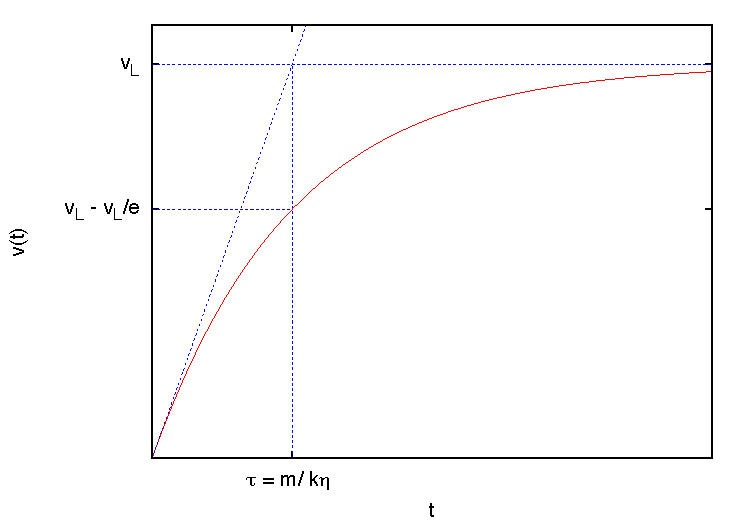
\includegraphics[width=0.8\textwidth]{./plote}
	\caption{ Evolução da velocidade de um corpo em queda livre sujeito a uma força de atrito. \label{fig:vLim}} 
\end{figure}

e quando $t \to \infty :\; v(t) \to v_L = \frac{m\,g}{k  \, \eta} $

Se pretendermos ser mais rigorosos devemos substituir  em (\ref{eq:vlimit}) o peso do corpo pelo seu “peso aparente” no fluido. Isto é, quando um corpo cai em queda livre através de um fluido, sofre além da acção da força de atrito outra força de baixo para cima devida ao princípio de Arquimedes, igual ao peso do fluido deslocado pelo corpo. Então o peso real do corpo deverá ser substituído pelo seu “peso aparente” no fluido e as equações (\ref{eq:mov}) e (\ref{eq:vlimit}) deverão ser modificadas para:

\begin{equation}
	\label{eq:mov2}
	m\,a = m\,g - m_f\,g  - k  \, \eta \, v
\end{equation}


\begin{equation}
	\label{eq:vlimit2}
	v_L = \frac{(m - m_f)\,g}{k  \, \eta}
\end{equation}

Sendo $m_f$ a massa do fluido deslocado.

No caso de um corpo esférico de raio R, introduzindo a equação (\ref{eq:coef_atrito}) em (\ref{eq:vlimit2}) e atendendo a que:
\begin{equation*}
	m = \frac{4}{3} \pi R^3 \rho \quad \textrm{  e } \quad  m_f = \frac{4}{3} \pi R^3 \rho_f
\end{equation*}

Obtemos:
\begin{equation}
	\label{eq:vlimit3}
	v_L = \frac{2\,R^2\, (\rho - \rho_f)\,g}{9  \, \eta}
\end{equation}

em que $\rho$  e $\rho_f$ são as massas específicas do corpo e do fluido.

%
\subsection{\sf Equilíbrio dum corpo num fluido não condutor, através de uma força eléctrica.}

\begin{figure}
	[!htb]  \centering 
	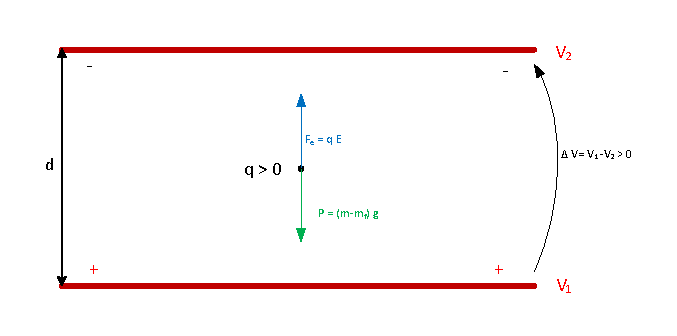
\includegraphics[width=0.8\textwidth]{./F_equil}
	\caption{Equilíbrio de forças eléctrica e gravítica \label{fig:f_equil}} 
\end{figure}

Seja o esquema representado na figura \ref{fig:f_equil}, em que entre duas placas condutoras paralelas se encontra um fluido não condutor. Aplica-se uma diferença de potencial $\Delta V = V_1 -V_1 > 0$ com a polaridade indicada na figura. Esta diferença de potencial criará um campo eléctrico de baixo para cima. No caso de entre as duas placas se encontrar uma partícula de massa m e de carga q positiva\footnote{No caso da partícula estar carregada negativamente obteríamos o mesmo resultado invertendo o sentido do campo eléctrico.} esta ficará sujeita a uma força eléctrica que contrariará a sua queda.

No caso de entre as placas se poder considerar o campo eléctrico (  ) como uniforme o seu módulo será dado por:


\begin{equation*}
	E = \frac{\Delta\, V}{d}
\end{equation*}
sendo $d$ a distância entre as placas. O módulo da força eléctrica que actua a partícula será então  dado por: 

\begin{equation*}
	F = |q| \frac{\Delta V}{d}
\end{equation*}

Deste modo a queda da partícula será agora contrariada, pela força de atrito e pela força eléctrica. A equação (\ref{eq:mov2}) passa a escrever-se:

\begin{equation}
	\label{eq:mov3}
	m\,a = (m - m_f)\,g  - q \frac{\Delta\, V}{d} - k  \, \eta \, v
\end{equation}

Variando a d.d.p. $\Delta V$ pode-se estabelecer o equilíbrio entre o peso da partícula e a força eléctrica, conseguindo-se a sua paragem entre as placas. Nesse caso será $a=0$ e $v=0$ e tem-se:

\begin{equation}
	\label{eq:equil}
	0 = (m - m_f)\,g  - q \frac{\Delta\, V}{d} 
\end{equation}

Substituindo em (\ref{eq:equil}) $(m - m_f)\,g$   pela equação (\ref{eq:vlimit2}) obtemos:

\begin{equation*}
	v_L\, k\, \eta = q \frac{\Delta\, V}{d}
\end{equation*}

E entrando também com (\ref{eq:coef_atrito}) no caso de a partícula ser esférica, obtemos:

\begin{equation}
	\label{eq:carga}
	q = \frac{6 \pi \, R \, \eta \, d\, v_L}{\Delta V}  
\end{equation}

Onde

\begin{itemize}
\item $v_L$, a velocidade limite de queda da partícula através do fluido na ausência do campo eléctrico. 
\item $\eta = 18.5 \times 10^{-5} P =  18.3 \times 10^{-6} \; Pa\times s $ (viscosidade do ar a 23ºC).
\item $\rho = 973 kg\,m^{-3}$ ( massa específica do óleo de silicone).
\item $\rho_f = 1 kg\,m^{-3}$ ( massa específica do ar).
\item $g=9.800\, m^{-1}\,s^{-2}$ ( Aceleração gravítica em Lisboa).
\item $d=5.0\, mm$ ( distância entre placas).
\end{itemize}

\subsection{\sf Correcções.}
\subsubsection{\sf Temperatura Ambiente.}

O valor da densidade da viscosidade do ar, no caso da temperatura ambiente se afastar muito de 23 ºC, terá de ser corrigido\footnote{Utilize por exemplo a caculadora \emph{online}: http://www.lmnoeng.com/Flow/GasViscosity.htm}

\subsubsection{\sf Dimensão das gotas.}

A Lei de Stokes não é exacta quando as dimensões dos corpos esféricos forem comparáveis às distâncias entre as moléculas do fluido (ar).
Nestas condições Millikan verificou que a viscosidade $\eta$ deveria ser substituída por

\begin{equation}
	\label{eq:correcao}
	\eta' = \frac{\eta}{1 + b/(p\,R)}  
\end{equation}

em que $b$ é uma constante igual $0.000617$, $p$ é pressão expressa em $cm$ de mercúrio\footnote{$1\,atm  = 1.013 \times 10^5 \,Pa = 1013 \, mbar = 76\, cm_{Hg}$}  e $R$ é o raio da gota em $cm$.

O valor corrigido $q_c$ pode ser determinado afectando o valor experimental $q$ por

\begin{equation}
	\label{eq:correcao1}
	q ' = q\, \left(\frac{\eta'}{\eta}\right)^{3/2}  =q\, \left(\frac{1}{1 + b/(p\,R)}\right)^{3/2}  
\end{equation}

\newpage
\section{\sf Procedimento Experimental}

\subsection{\sf Material utilizado}

\begin{enumerate}
	\item Célula de Millikan com gerador de alta tensão (DC) regulável (potenciómetro) 
	\item  Atomizador e óleo de silicone 
	\item Multímetro 
	\item Cronómetro 
	\item Nível de bolha de ar 
	\item Parafuso de calibração do retículo do microscópio
\end{enumerate}
\section{\sf Procedimento experimental}

\begin{enumerate}
\item   Depois de verificar que a célula está horizontal e colocando o potenciómetro que 
controla a alimentação das placas do condensador no valor mínimo de tensão electrica,
focalize o microscópio. Observe se o orifício que as gotículas atravessam está 
desobstruído.
\item    Verifique se o interruptor de inversão da alimentação do condensador está desligado.
Rode o potenciómetro para uma posição que permita quando o interruptor de inversão
estiver ligado estabelecer um campo eléctrico entre as placas do condensador. 
\item     Utilizando o pulverizador junto do orifício da célula produza uma pequena “nuvem”
de gotículas de óleo. Observe através do microscópio o movimento das gotículas em 
frente do retículo (a imagem encontra-se invertida).
\item     Variando a intensidade do campo eléctrico aplicado ao condensador por meio do 
potenciómetro verifique se as gotículas estão electrizadas. Inverta o sentido do campo 
eléctrico. Escolha uma das gotas.
 \item Obrigue a gota a colocar-se numa determinada divisão do retículo, imobilizando-a. 
Leia o valor da diferença de potencial que permitiu essa imobilização. Interrompa o 
campo eléctrico e verá a gota movimentar-se (com velocidade limite). Com um 
cronómetro meça o tempo necessário para que a gota faça um percurso de N divisões
do retículo. Repita pelo menos duas vezes. Repita este processo para várias gotas (pelo 
menos cinco). 
\item   Calcule a velocidade limite média de cada gota e respectiva incerteza. Estime o raio e 
a carga de cada gota e correspondentes incertezas. Verifique se se justifica considerar 
que a gotícula se move com velocidade limite 
\item   Compare os valores das cargas obtidas com o valor da carga do electrão.
\end{enumerate}

Critique a precisão dos resultados obtidos. Discuta a partir dos resultados obtidos e atendendo
aos erros experimentais se é possível concluir sobre a quantificação da carga eléctrica.

\end{document} 